%%%%%%%%%%%%%%%%%%%%%%%%%%%%%%%%%%%%%%%%%%%%%%%%%%%%%%%%%%%%%%%%%%
%  Thesis template file  prepared by:
%  Thyge Kn�ppel, tkn@elektro.dtu.dk, DTU Elektro, May 2008
%  Based on the work of Jan Larsen, IMM, DTU (cf. http://www2.imm.dtu.dk/teaching/phd/)
% 
%  CET June 2010 edited Charlotte K. Madsen
%%%%%%%%%%%%%%%%%%%%%%%%%%%%%%%%%%%%%%%%%%%%%%%%%%%%%%%%%%%%%%%%%%

%Hand-in code: 4282

%%%%%% Compilation: 
% compilation using latex (i.e. via a ps file)
%\documentclass[a4paper,11pt,twoside,openright,dvips]{book}

% compilation using PDFLATEX - Note that pdflatex is known to have issues with
% some of the pstricks-packages
\documentclass[a4paper,11pt,twoside,openright,pdftex]{book}
%%%%%%%%%%%%%%%%%%%%%%%%%%%%%%%%%%%%%%%%%%

%%%%%%%%%%%%%%%%%%%%%%%%%%%%%%%%%%%%%%%%%%%%%%%%%%%%%%%%%%%%%%%%%%
% Input information for cover, titlepages:
% Sould be EDITED to match your work!

\def\ThesisAuthor{Elvar Orn Unnthorsson, 101403}%multiple authors separated by "\\"
                         %If there are multiple authors adjust the \vspace 
                         %in thesislayout.sty as necessary
\def\ThesisAuthorForHyperref{Elvar Orn Unnthorsson, 101403}%list of authors for pdf
                                %properties. Multiple authors separated by ","
\def\ThesisTitle{Sentiment Analysis Of\\ Football Tweets} %project title
\def\Subtitle{02820 Python Programming} %subtitle - if any
\def\thesiskeywords{Twitter, Tweets, Sentiment, Analysis, Football} %keywords for the pdf file
\def\thesissubject{} %only for pdf properties - doesn't appear on printed
                     %versions
\def\Supervisor{Supervisor 1\\Supervisor 2} %list of supervisors. multiple
                                %supervisors are separated by "\\"
\def\projecttype{7. December 2011} %type of project (see README file
                                %for explanation)
\def\ISBNNUMBER{} %type \ISBNNUMBER{ISBN: xxx} if your project has one
\def\DatePublished{Date published} %date of publication
\def\Klasse{1 (public)} %project class (see README file for explanation)
\def\Degree{Master of Science in Digital Media} %obtained degree (see
                                                %README file for explanation)
\def\ECTSpoints{30} %# of ECTS points 
\def\Udgave{First} %edition
\def\Owner{Elvar Orn Unnthorsson, 2011} %name of copyright and year
%%%%%%%%%%%%%%%%%%%%%%%%%%%%%%%%%%%%%%%%%%%%%%%%%%%%%%%%%%%%%%%%%%

%%%%%%%%%%%%%%%%%%%%%%%%%%%%%%%%%%%%%%%%%%%%%%%%%%%%%%%%%%%%%%%%%%
%%%%%%%%%%%%% Change settings: (compile twice )%%%%%%%%%%%%%%%%%%%%%%
\def\thesisversion{final} %OBS: choose this for final version (official set of
                          %title pages) 
%\def\thesisversion{draft} %OBS: choose this for draft version (simple title
                           %page and no info page)

\def\thesislinks{no}%OBS: choose this for paper version (no colored links) 
%\def\thesislinks{yes}%OBS: choose this for online version (with links)
%%%%%%%%%%%%%%%%%%%%%%%%%%%%%%%%%%%%%%%%%%%%%%%%%%%%%%%%%%%%%%%%%%

%%%  For changing language: (compile twice -first time gives errors)%%%
\def\thesislanguage{en} %OBS: compile document for English 
%\def\thesislanguage{da}  %OBS:  compile document for Danish


%%%%%%%%%%%%%%%%%%%%%%%%%%%%%%%%%%%%%%%%%%
% Load style definitions, packages, etc:
	\usepackage{style/thesisdef} 		% packages  listings aso
	\usepackage{style/thesislayout} 	% layout; headings, pagemargin, theorems aso
	\usepackage{style/Mythesis} 	  	% Locals editings to only your thesis
%%%%%%%%%%%%%%%%%%%%%%%%%%%%%%%%%%%%%%%%%%
% END of premable
%%%%%%%%%%%%%%%%%%%%%%%%%%%%%%%%%%%%%%%%%%%%%%%%%%%%%%%%%%%%%%%%%%

%%%%%%%%%%%%%%%%%%%%%%%%%%%% DOCUMENT %%%%%%%%%%%%%%%%%%%%%%%%%%%%
\begin{document}

%%%%%%%%%%%%%%%%% Edit ONLY for printing type:
% Front matter:
	\frontmatter

  \ifx\thesisversion\printversion
	% for final version include standard dtu cover pages
	\pagenumbering{alpha}%dummy numbering for pdf-file (numbering set as a
                    %pdf-property and is NOT visible on the document). The
                    %hyperref package complains if duplicate numbering exists
	\coverpages    %generates the first four pages (thesislayout.sty)
	\else
%for draft version use simple title page:
	\title{\ThesisTitle{} - \Subtitle{}}
	\author{\ThesisAuthor}
	\thispagestyle{empty}
	\maketitle
	%\clearpage{\thispagestyle{empty}\cleardoublepage}
   \fi
%%%%%%%%%%%%%%%%%%%%%%%%%%%%%%%%%%%%%%%%%%

%%%%%%%%%%%%%%%%%%%%%%%%%%%%%%%%%%%%%%%%%%%%%%%%%%%%%%%%%%%%%%%%%%
% PREFACE CHAPTERS INCLUDE: files are in folder "file"
	\pagenumbering{roman}
	\pagestyle{empty} 	%For first few pages %\markboth{}{}
	
%  \ifx\thesisversion\printversion % no resumes in draft-version
%% Ad to List of Contents:
%\chapter*{Abstract, Resum�}
%	\ifx\thesislanguage\danishlang
%	\addcontentsline{toc}{chapter}{Resum�}
%	\else
%	\addcontentsline{toc}{chapter}{Abstract}
%	\fi
%\input{file/abstract}

%% Ad to List of Contents:
%\chapter*{Resum�, Abstract}
%	\ifx\thesislanguage\danishlang
%	\addcontentsline{toc}{chapter}{Abstract}
%	\else
%	\addcontentsline{toc}{chapter}{Resum�}
%	\fi
%\input{file/resume}
%  \fi

% if a chapter is wanted BEFORE lists
%% Ad to List of Contents:
%\chapter*{Preface, Forord}
%	\ifx\thesislanguage\danishlang
%	\addcontentsline{toc}{chapter}{Forord}
%	\else
%	\addcontentsline{toc}{chapter}{Preface}
%	\fi
%\input{file/preface} %lines above can be moved into this file
%%%%%%%%%%%%%%%%%%%%%%%%%%%%%%%%%%%%%%%%%%%%%%%%%%%%%%%%%%%%%%%%%%

%%%%%%%%%%%%%%%%%%%%%%%%%%%%%%%%%%%%%%%%%%
% TOC,LOF,LOT and SETUP HEADER: (should not be edited)
	\pagestyle{fancyplain}		%'plain' enable center-food-pagenumber only
							%'fancyplain' gives right-left numbers
	%\cleardoublepage 
	\phantomsection  	% makes pdf-hyperref work in adobe
	\addcontentsline{toc}{chapter}{Table Of Contents}
\tableofcontents  
\clearpage
\pagenumbering{arabic}
%  \ifx\thesisversion\printversion	
%	\cleardoublepage 	\phantomsection  	% makes pdf-hyperref work in adobe
%	\ifx\thesislanguage\danishlang
%	\addcontentsline{toc}{chapter}{Figurliste}
%	\else
%	\addcontentsline{toc}{chapter}{List of Figures}
%	\fi
%\listoffigures

%	\cleardoublepage 	\phantomsection  	% makes pdf-hyperref work in adobe
%	\ifx\thesislanguage\danishlang
%	\addcontentsline{toc}{chapter}{Tabelliste}
%	\else
%	\addcontentsline{toc}{chapter}{List of Tables}
%	\fi
%\listoftables
%  \fi
%%%%%%%%%%%%%%%%%%%%%%%%%%%%%%%%%%%%%%%%%%

\label{fancy:frontend} %for 'of page /x'
%\clearpage{\thispagestyle{empty}\cleardoublepage}

%%%%%%%%%%%%%%%%%%%%%%%%%%%%%%%%%%%%%%%%%%%%%%%%%%%%%%%%%%%%%%%%%%
% MAIN CHAPTERS INCLUDED FROM FOLDER  "file":
	\mainmatter 
	\setcounter{page}{1}
	\pagenumbering{arabic}
	\pagestyle{fancytext}

% if a chapter is wanted after lists or other unnumbered chapter
%% Ad to List of Contents (can also be the first entry after \chapter in the file:
%	\cleardoublepage 
%	\phantomsection
%	\addcontentsline{toc}{chapter}{Introduction}
%	\markboth{Preface}{}
%\input{file/introduction} 

%The report could contain, e.g.:
%Discussion of the design of the program
%Description of the implementation.
%Table or graphical overviews of modules and/or classes
%Database schema description
%Description of central parts of the code
%Screenshots of the program
%Plots of results
%Plots of code performance


%%%%%%%%%%%%%%%%%%%%%%%%%%%%%%%%%%%%%%%%%%%%%%%%%%%%%%%%%
\chapter[Introduction]{Introduction}
\label{chap:Introduction}

This report describes in detail the design and implementation of the final project done for the course 02820 Python Programming.\\

There have been many projects that try to do sentiment analysis of text but, to the best of the author's knowledge, 
none have focused on football related comments and tweets from fans of the sport. It seemed ideal to the author to 
look at that area and see if he could create a program that can see if fans are speaking positively or negatively 
towards players, teams, managers, referees, something that happens in a game etc.\\

The main goal of the project was to a create a program that collects football related comments and tweets from Twitter,
perform a sentimental analysis of of each tweet collected and to show the results by creating a webpage. The program was
written with the Python programming language, uses the Twitter GET Search API to collect tweets, performs the analysis 
using Naive Bayes Classifier and displays the results in a simple html webpage.\\ 

An additional feature was to try to put collected data in a database. This is beneficial as the program can easily fetch
old data, for searches that have already been done before, and use it with the newly harvested tweets.\\

The work for this project was done between 29.August and 7.December in the fall semester of 2011.

\setcounter{page}{2}
%%%%%%%%%%%%%%%%%%%%%%%%%%%%%%%%%%%%%%%%%%%%%%%%%%%%%%%%%
\chapter[Design of the program]{Design of the program}
\label{chap:design_of_the_program}

This chapter focuses on the program's design and thoughts behind it.\\

From the beginning the author knew that he wanted to accomplish three things:
\begin{itemize}
	\item Harvest tweets
	\item Analyze the harvested tweets
	\item Display the results
\end{itemize}

So it naturally made sense to create separate classes for each of those tasks. The author also decided to
create a main class for the program, whose task would be to call the other classes with appropriate parameters
and display the program's status during runtime. Then for the additional feature, to save the tweets collected
in a database, it seemed only natural that the class responsible for the tweet harvesting should be the one that
saves the data and offers other classes access to the data to the database.\\

After looking at a few database solutions the author decided to use the Redis solution because of its simplicity
and ease of use and also to minimize time required for the author to familiarize with the solution since he had
used Redis in a different DTU course this semester.\\

The program therefore consists of four separate Python classes and a Redis database. Each module servers a specific 
purpose in order to accomplish the program's objective. Section 2.4 shows the class overview.

\section{Class FootballAnalyzer} \label{sec:FootballAnalyzerDesign}
The FootballAnalyzer class is the main class in the program and gives other classes the parameters needed 
and receives the data from them. It also displays on the command line the progress of the search, analysis
and html creation. 

\section{Class TwitterAggregator} \label{sec:TwitterAggregatorDesign}
The TwitterAggregator purpose is to search Twitter for tweets, get and save the relevant data to a database
and offer other classes the chance to retrieve the tweet data that has been harvested.

\section{Class SentimentAnalyzer} \label{sec:SentimentAnalyzerDesign}
The SentimentAnalyzer's job is to create a Naive Bayes classifier that uses manually analyzed data, created
by the author, to train how to recognize positive, negative and neutral tweets. The class then takes a list
of tweets and performs a sentiment analysis to classify them into appropriate categories and returns a list
with the classification information appended to the list.

\section{Class HTMLCreator} \label{sec:HTMLCreatorDesign}
The HTMLCreator is the class responsible for creating the web page that displays the results from the football
analyzer. It takes a dictionary of statistics gathered while harvesting and analyzing the tweets and a list of 
all tweets analyzed in the run of the program. \\

The class then displays the statistics, creates a word cloud of the most popular words used in the tweets and
lists every tweet sent to it, colored in a way so that it is easy to see how the classifier classified each
tweet that it was give.

\section{Overview} \label{sec:ClassOverview}
\begin{figure}[ht]
	\centering
		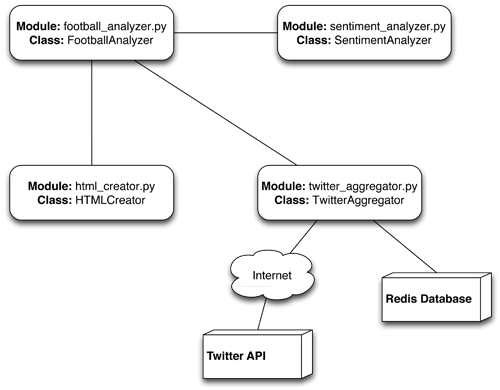
\includegraphics[height=330px]{images/ClassOverview.png}
	\caption{ Class overview of the football analyzer }
	\label{fig:images_ClassOverview}
\end{figure}
%%%%%%%%%%%%%%%%%%%%%%%%%%%%%%%%%%%%%%%%%%%%%%%%%%%%%%%%%
\chapter[Implementation]{Implementation}
\label{chap:Implementation}

This chapter focuses on how the classes and database were implemented in to the system.

\section{Class FootballAnalyzer} \label{sec:FootballAnalyzerImplementation}
FootballAnalyzer has the following functions:\\

{\bf Public}
\begin{itemize}
\item run( self )
\end{itemize}

{\bf Private}
\begin{itemize}
\item \_\_search( self )
\item \_\_analyze( self, tweets )
\item \_\_create\_webpage( self, analyzed\_tweets )
\item \_\_start\_task( self )
\item \_\_end\_task( self )
\item \_\_print\_time( self, delay )
\end{itemize}

The FootballAnalyzer creates an instance of the TwitterAggregator to get the tweets defined in the search parameters. It then creates an instance of the SentimentAnalyzer and makes it analyze all the tweets that were harvested from Twitter to get the sentiment classification of each tweet collected. \\

Finally it creates an instance of the HTMLCreator, sends the data from the aggregator and analyzer and makes it create a webpage that shows the results from the program.\\

To use the FootballAnalyzer you have define search terms and specify how many pages of tweets you want the class to search for and how many tweets should be on each page. With those parameters defined you can create an instance of the class and make it run by calling the run() function.\\

\clearpage

\section{Class TwitterAggregator} \label{sec:TwitterAggregatorImplementation}
FootballAnalyzer has the following functions:\\

{\bf Public}
\begin{itemize}
\item twitter\_search( self, search\_terms, pages, results\_per\_page )
\item get\_tweets( self, search\_terms, return\_all\_tweets )
\end{itemize}

{\bf Private}
\begin{itemize}
\item \_\_get\_tweet\_ids( self, search\_results )
\item \_\_is\_english\_tweet( self, tweet )
\end{itemize}

The TwitterAggregator performs a Twitter GET Search and harvests tweets using the search parameters given to it. It saves the twitter data, from the search, to a redis database and allows the user to get the data by calling the function "get\_tweets()".\\

Redis is a Key-Value type of database. The aggregator saves four different keys in the system. First it saves the search parameter, with spaces replaced by underscores, with the value True so it is easy to see if a search has been performed with those parameters. An example of this would be the key "Manchester\_United" and value "True". Next is saves a key with the search parameter and "\$TweetIds" appended to it and the value is a list of all tweet ids found in the search. Example of this is the key "Manchester\_United\$TweetIds" and value [u'143863607367700480', u'143863033024876544'...]. \\

To keep track of how many times a search has been performed in the program, the aggregator saves a key with the search parameter and "\$SearchCount" appended to it. Example is the key "Manchester\_United\$SearchCount" and value 5. Finally, to get the data from each tweet id, the aggregator saves each tweet id with the name "ID\$" and the id appended to the name. The value is a list which contains the tweet text, username and a URL to the profile picture of the user who created the tweet. An example would be the key "ID\$143863033024876544" and value ["Manchester United won today. Great!",\\ 'http://a1.twimg.com/sticky/default\_profile\_images/default\_profile\_2\_normal.png', 'velvetdismality']. \\

To use the TwitterAggregator you create an instance of the aggregator and call the twitter\_search() function with the search parameters, how many pages and number of tweets requested as parameters. Then to get the tweets collected, you call the get\_tweets() function with the search terms you want data from and True or False depending on whether you want all tweets with that search term or just the tweets harvested in the last run.\\

\section{Class SentimentAnalyzer} \label{sec:SentimentAnalyzerImplementation}
FootballAnalyzer has the following functions:\\

{\bf Public}
\begin{itemize}
\item analyze( self, data )
\item get\_analysis\_result( self, data\_to\_get )
\item show\_most\_informative\_features( self, amount )
\end{itemize}

{\bf Private}
\begin{itemize}
\item \_\_init\_naive\_bayes( self )
\item \_\_check\_word( self, word )
\item \_\_analyze\_tweet( self, tweet )
\item \_\_analyse\_using\_naive\_bayes( self, data )
\end{itemize} 

The SentimentAnalyzer uses the Naive Bayes classifier, that is included in the Natural Language toolkit, to classify tweets. It trains the classifier so that it can determine whether a tweet is positive, negative or neutral. The class opens up three different files, titled "tweets\_positive", "tweets\_negative", "tweets\_neutral", gets the text and places it in the classifier. The training data used that was manually categorized by the author and contains over 700 lines of words and sentences. The data was taken from Tweets harvested while creating the program and from football message boards. \\

When doing an analysis the SentimentAnalyzer removes known stop-words, all links found and words that have less than 3 letters. It does so by calling the check\_word() function, for each word, to see if it should include the word or not.\\

To use the SentimentAnalyzer one has to simply create an instance of it and send a list of tweets to the analyze() function which returns the list with each tweet classified.

\clearpage

\section{Class HTMLCreator} \label{sec:HTMLCreatorImplementation}
FootballAnalyzer has the following functions:\\

{\bf Public}
\begin{itemize}
\item create\_html( self )
\end{itemize}

{\bf Private}
\begin{itemize}
\item \_\_create\_stats\_info( self )
\item \_\_create\_tweet\_list( self )
\item \_\_create\_word\_cloud( self )
\end{itemize}

The HTMLCreator creates a HTML webpage that displays statistics, word cloud and a list of all tweets harvested. The class opens a html template which has all the markup for the webpage and stores it in a string. It takes the statistics given and puts them in a div element with the id "stats".\\

The HTMLCreator then creates a word cloud of the 30 most frequent words in the tweets found by the aggregator, each word within a <li></li> element with an appropriate css class and places them in the unordered list that has the class "word-cloud". The class for each word is determined by calculating how many times the word has appeared and scaled so that it is between 1 and 25.\\

The class then creates a list of tweets on the webpage. The webpage shows three tweets per line and assigns each tweet with the class "left-tweets" or "right-tweets" depending on where it should be shown. It also creates an extra div element to color the background of each tweet, green, red or white depending on the results from the classification from the SentimentAnalyzer. \\

A screenshot of the webpage can be seen in chapter 4.2.
%%%%%%%%%%%%%%%%%%%%%%%%%%%%%%%%%%%%%%%%%%%%%%%%%%%%%%%%%
\chapter[Results]{Results}
\label{chap:results}


\section{Most Informative Features} \label{sec:MostInformativeFeatures}

After training the Naive Bayes classifier with the manually categorized tweets and comments, the author
asked the classifier to show the 20 most informative features for it to recognize whether some text
should be classified positive, negative or neutral. Table 4.1 shows the results from the classifier.  \\

\begin{table}[h]
	\begin{center}
		\begin{tabular*}{10cm}{@{\extracolsep{\fill}} | r @{\hspace{1cm}} r @{\hspace{1cm}} l l r |  }
			\hline
			\multicolumn{5}{|c|}{Most Informative Features} \\
			\hline
			1 & starting = True & neu : pos & = & 21.5 : 1.0\\
			2 & great = True & pos : neg & = & 19.9 : 1.0\\
			3 & best = True & pos : neg & = & 12.8 : 1.0\\
			4 & world = True & pos : neg & = & 12.4 : 1.0\\
			5 & crossing = True & neu : pos & = & 7.2 : 1.0\\
			6 & thought = True & pos : neg & = & 7.1 : 1.0\\
			7 & player = True & neu : neg & = & 6.6 : 1.0\\
			8 & class = True & pos : neg & = & 6.4 : 1.0\\
			9 & shit = True & neg : pos & = & 6.2 : 1.0\\
			10 & good = True & pos : neg & = & 5.1 : 1.0\\
			11 & better = True & pos : neg & = & 4.9 : 1.0\\
			12 & fucking = True & neg : pos & = & 4.4 : 1.0\\
			13 & flicks = True & pos : neg & = & 3.4 : 1.0\\
			14 & decision = True & neg : pos & = & 3.3 : 1.0\\
			15 & even = True & neg : pos & = & 2.7 : 1.0\\
			16 & much = True & neg : pos & = & 2.7 : 1.0\\
			18 & can't = True & neg : pos & = & 2.7 : 1.0\\
			19 & like = True & pos : neg & = & 2.6 : 1.0\\
			20 & least = True & pos : neg & = & 2.6 : 1.0\\
			\hline
		\end{tabular*}
	\end{center}
	\caption{ Most informative features from the manually categorized tweets }
\end{table}

\newpage
\section{Results webpage} \label{sec:ResultsWebpage}

Below is a screenshot taken of the webpage created after running the program with the search parameters "MUFC Basel" which refer to the English team Manchester United Football Club and the Swiss football club Basel. \\

\begin{figure}[h]
	\centering
		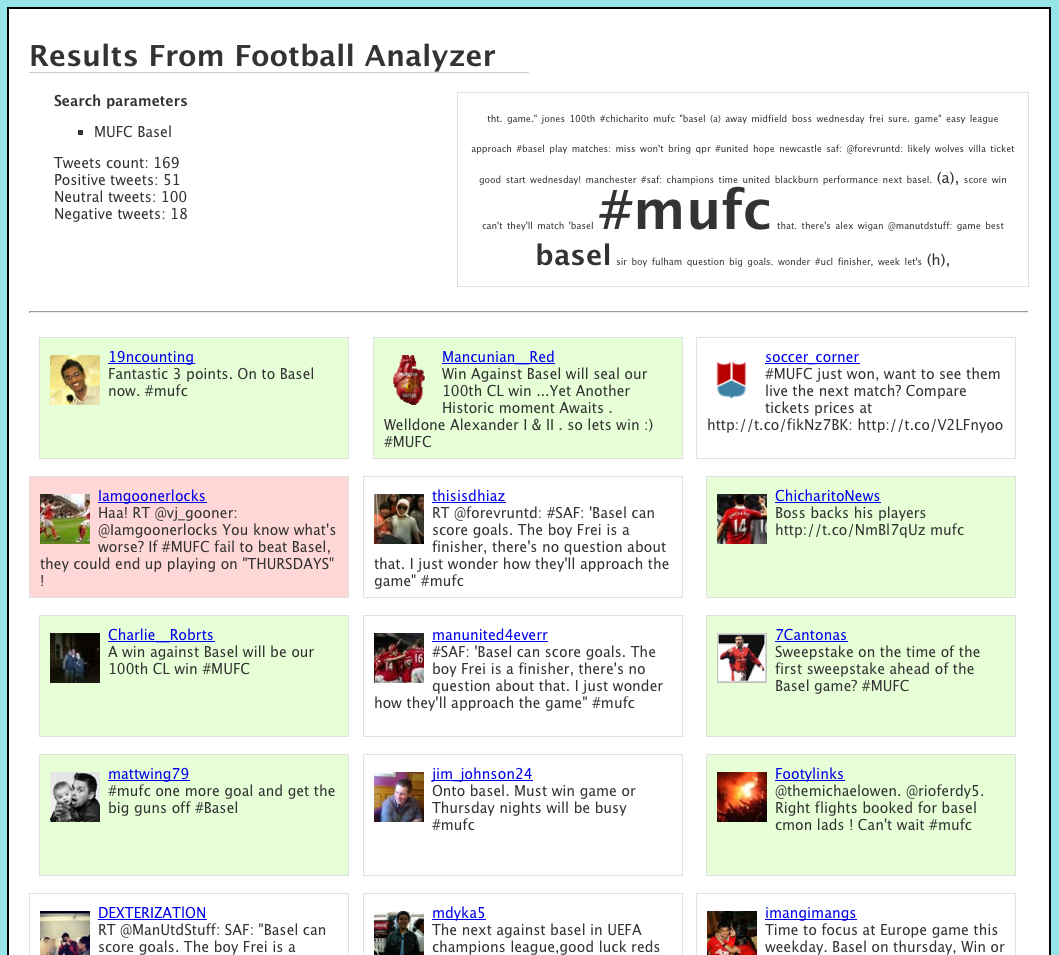
\includegraphics[width=400px]{images/webpage.png}
	\caption{ Screenshot of the results webpage }
	\label{fig:results}
\end{figure}

%To section \ref{sec:eqnom}


%%%%%%%%%%%%%%%%%%%%%%%%%%%%%%%%%%%%%%%%%%%%%%%%%%%%%%%%%%%%%%%%%%

%%%%%%%%%%%%%%%%%%%%%%%%%%%%%%%%%%%%%%%%%%
% BIBLIOGRAPHY: Build - bibtex to renew
%
%	\clearpage{\thispagestyle{empty}\cleardoublepage} \phantomsection 
%	\ifx\thesislanguage\danishlang
%	\addcontentsline{toc}{chapter}{Litteratur}
%	\else
%	\addcontentsline{toc}{chapter}{Bibliography}
%	\fi
%	\bibliographystyle{plainnat}
%\bibliography{bibbase}

%% Ad to Runin headings:
%	\ifx\thesislanguage\danishlang
%	\markboth{Litteratur}{}
%	\else
%	\markboth{Bibliography}{}
%	\fi
%%%%%%%%%%%%%%%%%%%%%%%%%%%%%%%%%%%%%%%%%%

%%%%%%%%%%%%%%%%%%%%%%%%%%%%%%%%%%%%%%%%%%%%%%%%%%%%%%%%%%%%%%%%%%
% APPENDIX:
\clearpage{\thispagestyle{empty}}%\cleardoublepage} 
\phantomsection 
\appendix	
\addcontentsline{toc}{chapter}{Appendix}

%%%%%%%%%%%%%%%%%%%%%%%%%%%%%%%%%%%%%%%%%%%%%%%%%%%%%%%%%
\chapter{ Poster for presentation }
\label{chap:appendix1}

A presentation was made for the project on the fifth of december in building 321. For the presentation it was required that the author made a presentation poster describing the program in a clear manner.\\

Figure A.1 shows the poster that was created for that presentation. \\

\begin{figure}[h]
	\centering
		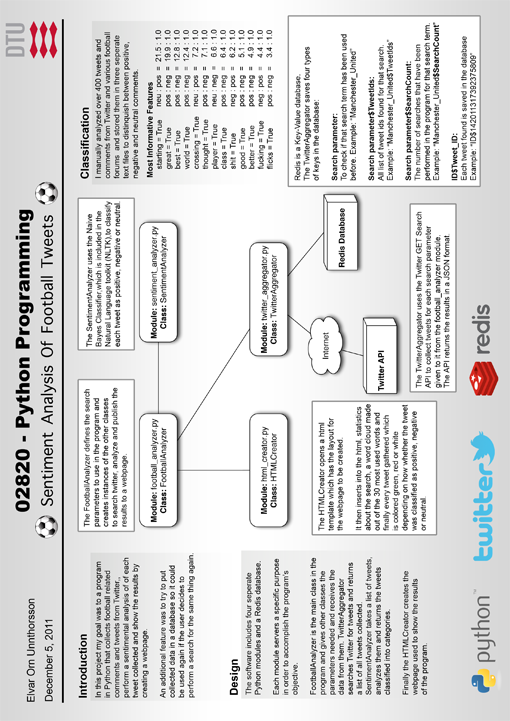
\includegraphics[height=515px]{images/Poster.png}
	\caption{ Presentation poster }
	\label{fig:images_Poster}
\end{figure}

%To section \ref{sec:eqnom}
\newpage
%%%%%%%%%%%%%%%%%%%%%%%%%%%%%%%%%%%%%%%%%%%%%%%%%%%%%%%%%
\chapter{ Program source code }
\label{chap:appendix2}

\section{football\_analyzer.py} \label{sec:FootballAnalyzer}
\begin{verbatim}
#!/usr/bin/env python
# encoding: utf-8
"""
twitter_sentiment_analysis.py

Created by Elvar Orn Unnthorsson on 07-12-2011
Copyright (c) 2011 ellioman inc. All rights reserved.
"""

import sys
import os
import twitter
import nltk
import thread
from twitter_aggregator import *
from html_creator import *
from sentiment_analyzer import *

class FootballAnalyzer:

  """
  FootballAnalyzer is searches twitter for tweets, performs a 
  sentiment analysis of each tweet harvested and creates a webpage,
  in the folder \"html\" that shows the results.
  """
  
  def __init__( self, search_terms = [], pages = 3, results_per_page = 50 ):
    """
    Input: search_terms. A list of search terms to for searching Twitter.
    Input: pages. A Number that determines how many pages of tweets to search for.
    Input: results_per_page. A Number which determines how many tweet results 
           should be on each page.
    Constructs a new FootballAnalyzer instance.
    """
    
    self.html_filename = "DataMiningResults.html"
    self.template_filename = "template.html"
    self.task_finished = False
    self.search_terms = search_terms
    self.pages = pages
    self.results_per_page = results_per_page
  
  
  def run( self ):
    """
    run( self ):
    Runs the football analyzer. Searches, analyzes and creates the webpage.
    """
    
    print "=======================\nData mining starting\n=======================\n"
    tweets = self.__search()
    analyzed_tweets = self.__analyze( tweets )
    self.__create_webpage( analyzed_tweets )
    
    print "=======================\nData mining successful\n=======================\n"
  
  
  def __search( self ):
    """
    __search( self ):
    Creates a search aggregator instance and performs a twitter search 
    using the the search parameters given in the constructor. Returns 
    a list of the tweets harvested.
    Return: A list of all tweets harvested.
    """
    
    try:
      print "Searching..."
      self.__start_task();
      self.aggregator = TwitterAggregator()
      self.aggregator.twitter_search( search_terms = self.search_terms, 
                                             pages = self.pages, 
                                  results_per_page = self.results_per_page )
      
      tweets = {} 
      for term in self.search_terms:
        tweets[term] = self.aggregator.get_tweets( search_terms = [ term ], 
                                                   return_all_tweets = True  )
      self.__end_task();
      print "Search complete"
      
      return tweets
    
    except:
      raise Exception ("Unknown error in FootballAnalyzer::__search")






  def __analyze( self, tweets ):
    """
    __analyze( self, tweets ):
    Input: tweets. A list of tweets strings
    Creates a sentiment analyzer instance and uses it to analyze each tweet 
    harvested by the twitter aggregator. it returns a list of the analyzed tweets.
    Return: A list of the tweets analyzed. 
    """
    
    try:
      print "Analyzing the data..."
      self.__start_task();
      self.analyzer = SentimentAnalyzer()
      analyzed_tweets = self.analyzer.analyze( tweets )
      self.__end_task();
      print "Analyzing complete"
      
      self.analyzer.show_most_informative_features( 20 )
      
      return analyzed_tweets
    
    except:
      raise Exception ("Unknown error in FootballAnalyzer::__analyze")
  
  
  def __create_webpage( self, analyzed_tweets ):
    """
    __create_webpage( self, analyzed_tweets ):
    Input: analyzed_tweets. A list of tweets strings
    Creates a webpage with statistics gathered from the tweet aggregator 
    and analyzer, a word cloud with the 30 most used words in the tweets
    and list of each tweet harvested which are colored green, red and white 
    depending on the results from the analyzer.
    """
    
    try:
      print "Creating HTML page..."
      self.__start_task();
      
      # A Statistic dictionary, 
      # used to print out the information on the results webpage.
      stats = {}
      stats["search_parameters"] = self.search_terms
      stats["tweets_count"] = self.aggregator.tweets_count
      stats["positive_count"] = self.analyzer.get_analysis_result( "positive" )
      stats["negative_count"] = self.analyzer.get_analysis_result( "negative" )
      stats["neutral_count"] = self.analyzer.get_analysis_result( "neutral" )
      

      html_page = HTMLCreator( self.html_filename, 
                               self.template_filename, 
                               analyzed_tweets, 
                               stats )
      html_page.create_html()
      self.__end_task();
      
      print "Creating HTML page complete\n"
    
    except:
      raise Exception ("Unknown error in FootballAnalyzer::__create_webpage")
  
  
  def __start_task( self ):
    """
    __start_task( self ):
    Creates a thread which displays dots while a function 
    in the FootballAnalyzer is running.
    """
    
    self.task_finished = False
    thread.start_new_thread( self.__print_time, ( 1.0, ) )
  
  
  def __end_task( self ):
    """
    __end_task( self ):
    Stops the thread created in the __start_task() function.
    """
    
    self.task_finished = True
    time.sleep( 1.0 )
  
  
  def __print_time( self, delay ):
    """
    __print_time( self, delay ):
    Input: delay. A number which determines how much time should be 
                  between the dot printing
    Prints dots while a function in the FootballAnalyzer is running.
    """
    
    while not self.task_finished:
      print "."
      time.sleep( delay )




if __name__ == '__main__':
  search = [ "MUFC LCFC", "Manchester United Liverpool" ]
  page_per_search = 3
  results_on_page = 300
  f = FootballAnalyzer( search_terms = search, 
                               pages = page_per_search, 
                    results_per_page = results_on_page )
  f.run()
\end{verbatim}

\section{twitter\_aggregator.py} \label{sec:TwitterAggregator}
\begin{verbatim}
#!/usr/bin/env python
# encoding: utf-8
"""
twitter_aggregator.py

Created by Elvar Orn Unnthorsson on 07-12-2011
Copyright (c) 2011 ellioman inc. All rights reserved.
"""

import string
import sys
import os
import re
import datetime
import twitter
import time
import redis
from os.path import join as pjoin
import ast


class TwitterAggregator:
  
  """
  TwitterAggregator performs a Twitter GET Search and harvests tweets
  using the search parameters given to it. It saves the twitter data,
  from the search, to a redis database and allows the user to get the
  data by calling the function "get_tweets()".
  """
  
  def __init__( self ):
    """
    Constructs a new TwitterAggregator instance.
    """
    
    self.redis = redis.Redis()
    self.info_to_get = ['text', 'profile_image_url', 'from_user']
    self.search_results = {}
    self.raw_data_directory_name = "raw_mining_data"
    self.filtered_data_directory_name = "filtered_mining_data"
    
    english_file = pjoin( sys.path[0], 
                          "sentiment_word_files", 
                          "Nielsen2010Responsible_english.csv")
    self.analyzeEnglish = dict(map(lambda (w,e): (w, int(e)), \
              [ line.strip().lower().split('\t') for line in open(english_file) ]))
    self.tweets_count = 0
  
  
  def twitter_search( self, search_terms = [], pages = 1, results_per_page = 100 ):
    """
    twitter_search( self, search_terms = [], pages = 1, results_per_page = 100 ):
    Input: search_terms. A list of search terms to for searching Twitter.
    Input: pages. A Number that determines how many pages of tweets to search for.
    Input: results_per_page. Number of tweets results on each page.
    Searches twitter for the things listed in the search_terms list and saves 
    the data collected, in a Redis database.
    """
    
    if search_terms == []: return ''
    
    self.pages = pages
    self.results_per_page = results_per_page
    twitter_search = twitter.Twitter( domain="search.twitter.com" )
    search_results = []
    
    try:
      # For each search term...
      for term in search_terms:
        results = []
        for page in range( 1, pages+1 ):
          results.append(twitter_search.search( q = term, 
                                              rpp = results_per_page, 
                                             page = page, 
                                      result_type = "recent" ) )
        
        # Get the tweets from the search
        new_tweets_ids = self.__get_tweet_ids( search_results=results )
        
        # Save tweets and other information to the database
        term_redis_name = term.replace( " ", "_" )
        term_tweetsIds_name = term_redis_name + "$TweetIds"
        term_searchcount_name = term_redis_name + "$SearchCount"
        


        if self.redis.exists( term_redis_name ):
          current_tweets_ids = ast.literal_eval( 
                                    self.redis.get( term_tweetsIds_name ) )
          current_tweets_ids.append( new_tweets_ids )
          self.redis.set( term_tweetsIds_name, current_tweets_ids )
          self.redis.set( term_searchcount_name, 
                          int( self.redis.get( term_searchcount_name ) ) + 1 )
        else:
          self.redis.set( term_redis_name, True )
          self.redis.set( term_tweetsIds_name, [new_tweets_ids] )
          self.redis.set( term_searchcount_name, 1 )
    
    except:
      raise Exception ("Unknown error in TwitterAggregator::twitter_search")
  
  
  def get_tweets( self, search_terms = [], return_all_tweets = True ):
    """ 
    get_tweets( self, search_terms = [], return_all_tweets = True ):
    Input: search_terms. A list of search terms to fetch from the database.
    Input: return_all_tweets. Boolean to say wether to get all or last tweets.
    Fetches from the database each tweet text, username and url to the user's 
    display pictures for each search term given in the "search_term" parameter.
    Return: A list which contains lists that has each tweet text, 
            username and url to profile picture.
    """
    
    returnList = []
    
    # If the search term list is empty, return an emptylist.
    if search_terms == []: return []
    
    try:
      # If not then get information about each tweet and put it in a list.
      for term in search_terms:
        term_redis_name = term.replace( " ", "_" )
        # Skip if the search term isn't in the database
        if not self.redis.exists( term_redis_name ): 
          print "Error: The search term", term, "has not been searched for before..."
          continue
        
        term_tweetsIds_name = term_redis_name + "$TweetIds"
        tweet_searches = ast.literal_eval( self.redis.get(term_tweetsIds_name) )
        
        if return_all_tweets:
          ids = list( set( [ t_id 
                             for results in tweet_searches 
                             for t_id in results ] ) )
          tweet_info = [ self.redis.get( t_id ) for t_id in ids ]
          
          for t in tweet_info:
            returnList.append( ast.literal_eval( t ) )
            self.tweets_count += 1
        
        else:
          ids = list( set( [ t_id 
                             for t_id in tweet_searches[ len(tweet_searches)-1 ] ] ) )
          tweet_info = [ self.redis.get( t_id ) for t_id in ids ]

          for t in tweet_info:
            returnList.append( ast.literal_eval( t ) )
            self.tweets_count += 1
      
      return returnList
    
    except:
      raise Exception ("Unknown error in TwitterAggregator::__get_tweet_ids")
      return []
  
  
  def __get_tweet_ids( self, search_results = [] ):
    """
    __get_tweet_ids( self, search_term = "", search_results = [] ):
    Input: search_results. A list with the JSON results from the Twitter API
    Fetches the tweet ids from the JSON results.
    Return: A list containing the ids found.
    """
    
    # Return empty list if the list in the parameter is empty
    if search_results == []: return []
    
    count = 0
    tweet_ids = []
    non_english_tweets = 0
    
    try:
      # For each search result...
      for result in search_results:
      
        # For each tweet found...
        for tweet in result['results']:
          # Skip tweets that are not in english
          if not self.__is_english_tweet( tweet['text'] ) :
            continue
            
          tweet_info = []


          # Get each information data that was requested...
          for fetched_data in self.info_to_get:
            if ( type(tweet[fetched_data]) == int): 
              tweet_info.append( tweet[fetched_data] )
            else: 
              tweet_info.append( tweet[fetched_data].encode('ascii', 'ignore') )
            
          # Append the information to the gathered list
          tweet_ids.append( tweet['id_str'] )
          
          # Put the tweet info in the database with the string ID as key
          self.redis.set( tweet['id_str'], tweet_info )
      return tweet_ids
    
    except:
      raise Exception ("Unknown error in TwitterAggregator::__get_tweet_ids")
      return []
  
  
  def __is_english_tweet( self, tweet ):
    """
    __isEnglishTweet( self, tweet ):
    Input: tweet. A string containing a tweet to check.
    Determines whether a comment is an english one or not. This function 
    was given to the author by Helgi who is a fellow student at DTU.
    Return: True if english, False if not not english
    """
    
    try:
      lang = sum(map(lambda w: self.analyzeEnglish.get(w, 0), \
        re.sub(r'[^\w]', ' ', string.lower(tweet)).split()))
        
      if lang >= 1.0: return True
      else: return False
    except:
      raise Exception ("Unknown error in TwitterAggregator::__isEnglishTweet")
      return False









\end{verbatim}

\section{sentiment\_analyzer.py} \label{sec:SentimentAnalyzer}
\begin{verbatim}
#!/usr/bin/env python
# encoding: utf-8
"""
sentiment_analyzer.py

Created by Elvar Orn Unnthorsson on 07-12-2011
Copyright (c) 2011 ellioman inc. All rights reserved.
"""

import sys
import os
from os.path import join as pjoin
import nltk
from nltk.classify import NaiveBayesClassifier
from nltk.corpus import stopwords
import codecs
import re

class SentimentAnalyzer:

  """
  SentimentAnalyzer trains a Naive Bayes classifier so that it can determine
  whether a tweet is positive, negative or neutral. It uses training data that
  was manually categorized by the author. The analyze function should be used
  to classify a list of tweets to analyze.
  """

  def __init__( self ):
    """
    Constructs a new SentimentAnalyzer instance.
    """

    self.results = { "positive": 0, "negative": 0, "neutral": 0}
    self.data = {}
    self.min_word_length = 3

    self.stopSet = set(stopwords.words('english'))
    extra_stopwords = ["he's", "she's", "RT" ]
    for stopword in extra_stopwords: self.stopSet.add( stopword )

    # Naive Bayes initialization
    self.__init_naive_bayes()





  def analyze(self, data):
    """
    analyze(self, data):
    Input: data. A list of tweets to analyze.
    Takes a list of tweets and uses sentiment analysis to determine whether 
    each tweet is positive, negative or neutral.
    Return: List with each tweet categorized with the proper sentiment value.
    """

    return self.__analyse_using_naive_bayes( data )


  def get_analysis_result(self, data_to_get):
    """
    get_analysis_result(self, data_to_get):
    Input: data_to_get. The statistic to get from the results dictionary.
    Gets the count of either positive, negative or neutral from the results 
    dictionary after doing an analysis. 
    Return: The count of positive, negative or positive tweets found.
    """

    return self.results[data_to_get]


  def show_most_informative_features( self, amount ):
    """
    show_most_informative_features( self, amount ):
    Input: amount. How many features should the function display.
    Displays the most informative features in the classifier used
    to classify each tweet.
    """

    self.classifier.show_most_informative_features( amount )


  def __init_naive_bayes( self ):
    """
    __init_naive_bayes( self ):
    Gets the data from the positive, negative and neutral text files.
    Creates and trains the Naive Bayes classifier, using the data, so 
    that it can learn what constitutes a positive, negative or neutral tweet.
    """

    try:
      pos_file = pjoin( sys.path[0], "sentiment_word_files", "tweets_positive.txt")
      f = codecs.open( pos_file, mode="rU", encoding='utf-8')
      positive = [ line.lower().replace("\n" , " ") for line in f ]
      positive = "".join(word[:] for word in positive).split()
      f.close

      neu_file = pjoin( sys.path[0], "sentiment_word_files", "tweets_neutral.txt")
      f = codecs.open( neu_file, mode="rU", encoding='utf-8')
      neutral = [ line.lower().replace("\n" , " ") for line in f ]
      neutral = "".join(word[:] for word in neutral).split()
      f.close

      neg_file = pjoin( sys.path[0], "sentiment_word_files", "tweets_negative.txt")
      f = codecs.open( neg_file, mode="rU", encoding='utf-8')
      negative = [ line.lower().replace("\n" , " ") for line in f ]
      negative = "".join(word[:] for word in negative).split()
      f.close

      posfeats = [( dict( { word.lower() : True } ), 'pos' ) 
                    for word in positive if self.__check_word( word ) ]
      neufeats = [( dict( { word.lower() : True } ), 'neu' ) 
                    for word in neutral if self.__check_word( word ) ]
      negfeats = [( dict( { word.lower() : True } ), 'neg' ) 
                    for word in negative if self.__check_word( word ) ]

      self.classifier = NaiveBayesClassifier.train( posfeats + neufeats + negfeats )

    except:
      raise Exception ("Unknown error in SentimentAnalyzer::__init_naive_bayes")
  
  
  def __check_word( self, word ):
    """
    __check_word( self, word ):
    Input: word. The word to check.
    Looks at a word and determines whether that should be used in the classifier.
    Return: True if the word should be used, False if not.
    """
    if word in self.stopSet \
      or len(word) < self.min_word_length \
      or word[0] == "@" \
      or word[0] == "#" \
      or word[:4] == "http":
        return False
    else:
      return True








  def __analyze_tweet(self, tweet):
    """
    __analyze_tweet(self, tweet):
    Input: tweet. The tweet that should be analyzed.
    Analyses a tweet using the created Naive Bayes classifier.
    Return: The results fromt the classifier. Possible results: 'pos', 'neg' or 'neu'
    """
    try:
      tweet_features = dict([ (word, True) 
              for word in tweet.lower().split() 
              if self.__check_word( word ) ] )
      return self.classifier.classify( tweet_features )
    
    except:
      raise Exception ("Unknown error in SentimentAnalyzer::__analyze_tweet")
      return 'err'


  def __analyse_using_naive_bayes(self, data):
    """
    __analyse_using_naive_bayes(self, data):
    Input: data. A list of tweets to analyze.
    Takes a list of tweets and uses sentiment analysis to determine 
    whether each tweet is positive, negative or neutral.
    Return: A list of the tweets analyzed.
    """
    analyzed_data = {}
    try:
      for search_term, tweet_data in data.iteritems():
        self.results[search_term + "_positive"] = 0
        self.results[search_term + "_negative"] = 0
        self.results[search_term + "_neutral"] = 0
        
        search_term_data = []
        for data in tweet_data:
          temp_data = data
          result = self.__analyze_tweet( data[0] )
          temp_data.append( result )
          search_term_data.append( temp_data )
          
          if (result == 'pos'): self.results[search_term + "_positive"] += 1
          elif (result == 'neg'): self.results[search_term + "_negative"] += 1
          elif (result == 'neu'): self.results[search_term + "_neutral"] += 1
        
        analyzed_data[search_term] = search_term_data
        self.results["positive"] += self.results[search_term + "_positive"]
        self.results["negative"] += self.results[search_term + "_negative"]
        self.results["neutral"] += self.results[search_term + "_neutral"]
      
      return analyzed_data
    
    except:
      raise Exception("Unknown error in SentimentAnalyzer::__analyse_using_naive_bayes")
      return analyzed_data
\end{verbatim}

\section{html\_creator.py} \label{sec:HTMLCreator}
\begin{verbatim}
#!/usr/bin/env python
# encoding: utf-8
"""
html_creator.py

Created by Elvar Orn Unnthorsson on 07-12-2011
Copyright (c) 2011 ellioman inc. All rights reserved.
"""

import sys
import os
import nltk
import random
from cgi import escape
from os.path import join as pjoin
from mako.template import Template


class HTMLCreator(object):

  """
  HTMLCreator creates a HTML webpage that displays statistics, word cloud
  and a list of all tweets harvested. Must provide the class with the following:
  * Name of the html page to create
  * Name of the template for the html to follow. The template must have: 
      * <ul id="cloud"> to place the word cloud
      * <div class="tweets"> to place the tweets
  * Twitter data consisting of list of [tweet text, profile pic, user name] lists
  """

  def __init__(self, page_name, template_name, twitter_data, stats):
    """
    Constructs a new HTMLCreator instance.
    """

    super(HTMLCreator, self).__init__()
    self.page_name = page_name
    self.template_name = template_name
    self.twitter_data = twitter_data
    self.tweets = ""
    self.word_cloud = ""
    self.stats_html = ""
    self.word_cloud_min_frequency = 5
    self.word_cloud_min_font_size = 1
    self.word_cloud_max_font_size = 25
    self.word_cloud_max_words = 30
    self.word_cloud_min_word_length = 3
    self.stats = stats


  def create_html(self):
    """
    create_html(self):
    Creates the webpage used to show the results 
    from the twitter search and analysis.
    """
    try: 
      f = open( pjoin(sys.path[0], "html/template", self.template_name), "r")
      html = f.read()
      f.close

      # Put the stats in the html
      self.__create_stats_info()
      index = html.find('<div id="stats">') + len('<div id="stats">')
      html_before_stats, html_after_stats = html[:index], html[index:]
      html = html_before_stats + self.stats_html + html_after_stats

      # Append the word cloud to the html
      self.__create_word_cloud()
      index = html.find('<ul id="cloud">') + len('<ul id="cloud">')
      html_before_cloud, html_after_cloud = html[:index], html[index:]
      html = html_before_cloud + '\n' + self.word_cloud + html_after_cloud

      # Append the tweets to the html
      self.__create_tweet_list()
      index = html.find( '<div class="tweet-container">')
                         + len('<div class="tweet-container">')
      html_before_tweets, html_after_tweets = html[:index], html[index:]
      html = html_before_tweets + self.tweets + html_after_tweets

      # Create and save the html file
      f = open( pjoin(sys.path[0], "html", self.page_name), "wb")
      f.write(Template("${data}").render(data=html))
      f.close()

    except:
      raise Exception ("Unknown error in HTMLCreator::create_html")


    def __create_stats_info(self):
      """
      __create_stats_info(self):
      Creates the statistics part of the webpage.
      """
      try:
        self.stats_html = '\n' + '\t'*6
        self.stats_html += '<strong>Search parameters</strong>\n'
        self.stats_html += '\t'*6 + '<br/>\n'
        self.stats_html += '\t'*6 + '<ul class="search-parameters">\n'

        for term in self.stats["search_parameters"]:
          self.stats_html += '\t'*7 + '<li>' + term + "</li>\n"

        self.stats_html += '\t'*6 + '</ul>\n'
        self.stats_html += '\t'*6 + 'Tweets count: '
        self.stats_html += str(self.stats["tweets_count"]) + '\n'
        self.stats_html += '\t'*6 + '<br/>\n'
        self.stats_html += '\t'*6 + 'Positive tweets: '
        self.stats_html += str(self.stats["positive_count"]) + '\n'
        self.stats_html += '\t'*6 + '<br/>\n'
        self.stats_html += '\t'*6 + 'Neutral tweets: '
        self.stats_html += str(self.stats["neutral_count"]) + '\n'
        self.stats_html += '\t'*6 + '<br/>'
        self.stats_html += '\t'*6 + 'Negative tweets: '
        self.stats_html += str(self.stats["negative_count"]) + '\n'
        self.stats_html += '\t'*6 + '<br/>'

      except:
        raise Exception ("Unknown error in HTMLCreator::__create_stats_info")


  def __create_tweet_list(self):
    """
    __create_tweet_list(self):
    Creates the tweet listing part of the webpage.
    """

    count = 1
    try:
      # For each result from the search...
      for search_term, results in self.twitter_data.iteritems():
        
        # For each tweet in the results...
        for tweet_data in results:
          
          # Make sure that the comments are in rows of three elements
          if ( count % 3 == 0 ):
            self.tweets += '\n' + '\t'*5 + '<div class="left-tweets">\n'
          else:
            self.tweets += '\n' + '\t'*5 + '<div class="right-tweets">\n'
          
          # See if it's a positive, negative or neutral tweet and 
          # put appropriate html class for the tweet
          if ( tweet_data[3] == "pos" ):
            self.tweets += '\t'*6 + '<div class="tweet-positive">\n'
          elif ( tweet_data[3] == "neg" ):
            self.tweets += '\t'*6 + '<div class="tweet-negative">\n'
          elif ( tweet_data[3] == "neu" ):
            self.tweets += '\t'*6 + '<div class="tweet-neutral">\n'
          
          # Image
          self.tweets += '\t'*7 + '<div class="img">\n' + '\t'*8
          self.tweets +='<img src="' + tweet_data[1] + '" width="50px"/>\n'
          self.tweets += '\t'*7 + '</div>\n'
          
          # Author's name
          self.tweets += '\t'*7 + '<div class="author">\n' + '\t'*8 
          self.tweets += '<a href="http://twitter.com/#!/' + tweet_data[2]
          self.tweets += '">' + tweet_data[2] + '</a>\n' + '\t'*7 + '</div>\n' 
          # Tweet text
          self.tweets += '\t'*7 + '<div class="text">\n' + '\t'*7 \
          self.tweets += tweet_data[0] + '\n' + '\t'*7 + '</div>\n' 
          self.tweets += '\t'*6 + '</div>\n'
          self.tweets += '\t'*5 + '</div>'
          
          if ( count % 3 == 0 ):
            self.tweets += '\n' + '\t'*5 + '<br class="clear">'
          count += 1

      self.tweets += '\n' + '\t'*5 + '<br class="clear">'

    except:
      raise Exception ("Unknown error in HTMLCreator::__create_tweet_list")


  def __create_word_cloud( self ):
    """
    __create_word_cloud( self ):
    Creates the word cloud part of the webpage. Takes the 30 most
    frequent words used and assigns the relevant class to it.
    Some of the code for this function was taken from the
    "the\_tweet\_tweet\_tagcloud\_code.py" from the book 
    "Mining the social web". The code can be found here on github:
     https://github.com/ptwobrussell/Mining-the-Social-Web
    """

    MIN_FREQUENCY = self.word_cloud_min_frequency
    MIN_FONT_SIZE = self.word_cloud_min_font_size
    MAX_FONT_SIZE = self.word_cloud_max_font_size
    MAX_WORDS = self.word_cloud_max_words
    MIN_WORD_LENGTH = self.word_cloud_min_word_length

    try:
      # Get all words from the tweet search and put them in a list
      tweets = []
      for search_term, results in self.twitter_data.iteritems():

        for tweet_data in results:
          tweet_words = tweet_data[0].split()

          # Append the words in lowercase to remove duplicates
          for word in tweet_words:
            tweets.append( word.lower() ) 

      # Compute frequency distribution for the terms
      fdist = nltk.FreqDist([term for t in tweets for term in t.split()])

      # Customize a list of stop words as needed
      stop_words = nltk.corpus.stopwords.words('english')
      stop_words += ['&', '&amp;', '.', '..','...','...', '?', '!']
      stop_words += [':', '"','&quot;', '(', ')', '()', '-', '--']
      stop_words += ["RT"] # Common Twitter words


      # Create output for the WP-Cumulus tag cloud and sort terms by freq
      raw_output = sorted([ [term, '', freq] for (term, freq) in fdist.items()
                  if freq > MIN_FREQUENCY 
                     and term not in stop_words 
                     and len(term) >= MIN_WORD_LENGTH], 
                  key=lambda x: x[2])

      # Scale the font size by the min and max font sizes
      # Implementation adapted from 
      # http://help.com/post/383276-anyone-knows-the-formula-for-font-s
      def weightTermByFreq(f):
        return (f - min_freq) \
               * (MAX_FONT_SIZE - MIN_FONT_SIZE) \
               / (max_freq - min_freq) + MIN_FONT_SIZE

      min_freq = raw_output[0][2]
      max_freq = raw_output[-1][2]
      weighted_output = [[i[0], i[1], weightTermByFreq(i[2])] for i in raw_output]

      # Create the html list <li> for the results page
      myList = []
      for (tag, n, font_size) in weighted_output:
        myList.append( '\t'*7 + '<li class="tag%d">%s</li>' % (font_size, tag) )



      # Minimize the html list to the number specified,
      # randomize it and add it to the word cloud string
      myList = myList[-MAX_WORDS:]
      random.shuffle(myList)
      self.word_cloud = '\n'.join(tag[:] for tag in myList)

    except:
      raise Exception ("Unknown error in HTMLCreator::__create_word_cloud")
\end{verbatim}
%\input{file/...}
%%%%%%%%%%%%%%%%%%%%%%%%%%%%%%%%%%%%%%%%%%%%%%%%%%%%%%%%%%%%%%%%%%

\label{fancy:mainend} %for 'of page /x'
%\clearpage{\thispagestyle{empty}\cleardoublepage}

%%%%%%%%%%%%%%%%%%%%%%%%%%%%%%%%%%%%%%%%%%
% BACK MATTER:
%	\backmatter
%	\ifx\thesisversion\printversion
%	\makebackpage %generates the backmatter (thesislayout.sty)
%	\fi
%%%%%%%%%%%%%%%%%%%%%%%%%%%%%%%%%%%%%%%%%%

\end{document}
